\documentclass[a4paper,polish,12pt]{article}
    \usepackage[utf8]{inputenc}
    \usepackage[T1]{fontenc}
    \usepackage{lmodern}
	\usepackage{amsmath}
	\usepackage{xcolor}
    \usepackage{babel}
    \usepackage{csquotes}
    \DeclareQuoteAlias{croatian}{polish}
    \usepackage[%
    style=verbose-ibid, % numeric, alphabetic, authoryear, ect.
    sorting=nty,
    isbn=false,
    abbreviate = false,
    backend=biber,]{biblatex}

    \renewcommand*{\newunitpunct}{\addcomma\space}
    \renewbibmacro*{in:}{}

    \usepackage{xpatch}

    \xpatchbibdriver{book}{%
    \newunit
    \iffieldundef{maintitle}
    {\printfield{volume}%
    \printfield{part}}
    {}%
    }
    {%
    }{}{}

    \xpatchbibdriver{book}{%
    \usebibmacro{publisher+location+date}%
    }
    {%
    \usebibmacro{publisher+location+date}%
    \newunit
    \printfield{volume}%
    \printfield{part}
    \usebibmacro{finentry}
    }{}{}

    \DeclareFieldFormat{journaltitle}{\mkbibquote{#1}}
    \DeclareFieldFormat[article,periodical]{number}{nr.  #1}% number of a journal

    \DeclareFieldFormat
    [article,inbook,incollection,inproceedings,patent,thesis,unpublished]
    {title}{\mkbibemph{#1}}
    %
    \renewbibmacro*{journal+issuetitle}{%
    \usebibmacro{journal}%
    \setunit*{\addspace}%
    \iffieldundef{series}
    {}
    {\newunit
    \printfield{series}%
    \setunit{\addspace}}%
    \usebibmacro{issue+date}%
    \setunit{\addspace}%
    \usebibmacro{issue}%
    \setunit{\addspace}%
    \usebibmacro{volume+number+eid}%
    \newunit}

    \renewbibmacro*{issue+date}{%
    \iffieldundef{issue}
    {\usebibmacro{date}}
    {\printfield{issue}%
    \setunit*{\addspace}%
    \usebibmacro{date}}%
    \newunit}

    \renewbibmacro*{publisher+location+date}{%
    \printlist{publisher}%
    \iflistundef{publisher}
    {\setunit*{\addcomma\space}}
    {\setunit*{\addcomma\space}}%
    \printlist{location}%
    \setunit*{\addspace}%
    \usebibmacro{date}%
    \newunit}
\usepackage{graphicx}
\usepackage{color}

\usepackage{listings}
 \renewcommand{\lstlistingname}{kod} %zmiana podpisu na polski

\definecolor{dkgreen}{rgb}{0,0.6,0}
\definecolor{gray}{rgb}{0.5,0.5,0.5}
\definecolor{mauve}{rgb}{0.58,0,0.82}


\lstset{frame=tb,
 language=Python,
 aboveskip=3mm,
 belowskip=3mm,
 showstringspaces=false,
 columns=flexible,
 basicstyle={\small\ttfamily},
 numbers=none,
 numberstyle=\tiny\color{gray},
 keywordstyle=\color{blue},
 commentstyle=\color{dkgreen},
 stringstyle=\color{mauve},
 breaklines=true,
 breakatwhitespace=true,
 tabsize=3
}

\usepackage{hyperref}
\newtheorem{theorem}{Twierdzenie}
\addbibresource{bik.bib}
\newtheorem{tw}{Twierdzenie}
\title{Projekt Cyfrowe przetwarzanie sygnałów}
\date{}
\author{Szymon Kozakiewicz}

\title{Dokumentacja}
\author{Mateusz banaszek \and Szymon Kozakiewicz \and Joanna Świętosławska}
\begin{document}
\maketitle
\tableofcontents
\section{Opis programu}
Program ma za zadanie udostępniać interfejs do komunikacji z full nodem sieci bitcoin. Pozawala na nawiązanie z nim połączenie oraz podstawową wymianę danych. Można więc uzyskać informacje o adresach innych węzłów czy otrzymać informacje o blokach i ich zawartości. Udostępnia też wysyłanie wiadomości czysto serwisowych takich jak ping, version czy verack. Możliwe są też różne sposoby na nawiązanie połączenia czyli UDP i TCP. 

\subsection{Realizowane funkcjonalności}

\begin{itemize}


\item Ustanowienie połączenia
\begin{itemize}
\item TCP
\item UDP
\end{itemize}

\item Komunikacja z użytkownikiem za pomocą konsoli
\item Znajdywanie adresów ip węzłów za pomocą DNS seed
\item Wysyłanie wiadomości:
\begin{itemize}
\item getaddr
\item addr
\item version
\item verack
\item ping
\item inv
\item getdata
\item getblocks
\end{itemize} 
\item Odbiór wiadomości
\begin{itemize}
\item addr
\item version
\item verack
\item ping
\item inv
\item tx

\end{itemize}
\end{itemize}

\subsection{Uruchomienie programu}
By uruchomić program należy wywołać polecenie $$python3 Console.py$$
Aplikacja była testowana dla pythona w wersji 3.6 na innych wersjach może on nie działać poprawnie.
\subsection{Opis działania}

Po uruchomieniu programu do konsoli można wpisać następujące polecenia:
\begin{itemize}
\item \textit{ping}:* wysyła wiadomość ping do wybranego hosta.
\item \textit{polacz}:* ustanawia połączenie z wybranym węzłem. Jeśli wcześniej żaden adres ip nie był ustawiony użytkownik zostanie poproszony o jego podanie. Wykonanie polecenia skutkuje wysłaniem do docelowego węzła wiadomości version. Następnie odebrana zostaje zwrotna wiadomość version od węzła. Na koniec następuje wymiana wiadomościami verack. Jeżeli nie uda się nawiązać połączenia TCP w przeciągu 5 sekund to próba połączenia kończy się niepowodzeniem.
\item \textit{help}:* Wyświetla możliwe do wpisania polecenia
\item \textit{ustaw adres}:* ustawia adres docelowego węzła
\item \textit{dns}:* wyszukiwanie adresów węzłów za pomocą dns. Wyszukane węzły zostają wypisane.
\item \textit{getaddr}: Wysyła wiadomość getaddr. Następnie odbiera wiadomość zwrotną addr która zawiera jeden lub więcej adresów ip węzłów
\item \textit{addr}: wysyła wiadomość addr do wybranego węzła
\item \textit{getblocks}:Wysyła wiadomośc getblocks do wybranego węzła. Następnie odbierana jest wiadomość inv, która zawiera informacje o blokach.
\item \textit{getdata}:  Wysyła wiadomość getdata do wybranego węzła. Następnie odbiera zwrotną wiadomość tx w, której zawiera informacje o transakcjach w bloku.
\item \textit{inv}: Wysyła wiadomość inv
\end{itemize}

Uwaga! Tylko polecenia oznaczone gwiazdką da się wykonać bez wcześniejszego nawiązania połączenia z węzłem(za pomocą polecenia \textit{polacz})

\section{Implementacja}
Aplikacja została stworzona przy użyciu języka \textit{python} w wersji 3.6. Nie były używane żadne zewnętrzne biblioteki.
\subsection{Opis konstrukcji poszczególnych wiadomości}

\subsubsection{Nagłówek wiadomości}
Każda wiadomość protokołu bitcoin musi rozpoczynać się od nagłówka. Składa się on z pól przedstawionych w tabeli \ref{tab:naglowek}
\subsubsection{Adres}
W wielu wiadomościach trzeba wysłać adres ip. Zawartość części wiadomości z adresem zaprezentowano w tabeli \ref{tab:addrInet}.
\begin{table}[]
\centering
\begin{tabular}{|l|c|c|}
\hline
\multicolumn{1}{|c|}{\textbf{nazwa pola}} & \textbf{liczba bajtów} & \textbf{komentarz}                                                                                                                                                                            \\ \hline
time                                      & 4                      & \begin{tabular}[c]{@{}c@{}}Czas. Pole nie jest obecne gdy \\ adres jest częścią wiadomości\\ version\end{tabular}                                                                             \\ \hline
services                                  & 8                      & -                                                                                                                                                                                             \\ \hline
ipv6/4                                    & 16                     & \multicolumn{1}{l|}{\begin{tabular}[c]{@{}l@{}}Pierwsze 12 bajtów przechowuje adres ipv6\\ pozostałe 4 bajty trzymają ipv4. W naszej\\ implementacji wykorzystujemy tylko ipv4.\end{tabular}} \\ \hline
port                                      & \multicolumn{1}{l|}{2} & \multicolumn{1}{l|}{Numer portu}                                                                                                                                                              \\ \hline
\end{tabular}
\caption{Zawartość adresu internetowego}
\label{tab:addrInet}
\end{table}

\subsubsection{Version}
Wiadomość version składa się z pól przedstawionych w tabeli \ref{tab:version}. Wiadomość wysyłana jest w celu ustalenia zasad komunikacji.

\begin{table}[]
\centering
\begin{tabular}{|l|c|l|}
\hline
\textbf{nazwa pola} & \textbf{liczba bajtów} & \textbf{Opis}                                                                                                                              \\ \hline
magic letters       & 4                      & \begin{tabular}[c]{@{}l@{}}Każda wiadomość rozpoczyna się od tzw \\ liczb magicznych.Zwykle mają \\ one postać f9beb4d9 (hex)\end{tabular} \\ \hline
command             & 12                     & Zawiera nazwę wiadomości                                                                                                                   \\ \hline
length              & 4                      & \begin{tabular}[c]{@{}l@{}}Długość wiadomości w \\ bajtach z pominięciem nagłówka\end{tabular}                                             \\ \hline
checksum            & 4                      & Suma kontrolna(przez nas nie odczytywana)                                                                                                  \\ \hline
\end{tabular}
\caption{Zawartość nagłówka wiadomości}
\label{tab:naglowek}
\end{table}


\begin{table}[]
\centering
\begin{tabular}{|l|c|c|}
\hline
\multicolumn{1}{|c|}{\textbf{nazwa pola}} & \textbf{liczba bajtów} & \textbf{Opis}                                                                                                                \\ \hline
version                                   & 4                      & \begin{tabular}[c]{@{}c@{}}Wskazuje wersje protokołu używaną\\ przez wysyłającego. W naszym wypadku \\ było to 60002\end{tabular} \\ \hline
services                                  & 8                      & -                                                                                                                                 \\ \hline
timestamp                                 & 8                      & czas wysłania wiadomości                                                                                                          \\ \hline
addr\_recv                                & 26                     & Adres adresata wiadomości                                                                                                         \\ \hline
addr\_from                                & 26                     & Adres wysyłającego                                                                                                                \\ \hline
nonce                                     & 8                      & -                                                                                                                                 \\ \hline
user\_agent                               & ?                      & -                                                                                                                                 \\ \hline
start\_height                             & 4                      & -                                                                                                                                 \\ \hline
relay                                     & 1                      & -                                                                                                                                 \\ \hline
\end{tabular}
\caption{Zawartość wiadomości version}
\label{tab:version}
\end{table}
\subsubsection{Verack}
Wiadomość składa się z samego nagłówka. Wysyłana jest w celu potwierdzenia nawiązania komunikacji.
\subsubsection{Getaddr}
Wiadomość składa się z samego nagłówka. Wysyłana jest w celu uzyskania nowych adresów ip węzłów.
\subsubsection{Addr}
Zawartość wiadomości addr została przedstwaiona w tabeli \ref{tab:addr}
\begin{table}[]
\centering
\begin{tabular}{|l|c|c|}
\hline
\multicolumn{1}{|c|}{\textbf{nazwa pola}} & \textbf{liczba bajtów} & \textbf{komentarz}                                                                                                                                                                                         \\ \hline
count                                     & 1+                     & \begin{tabular}[c]{@{}c@{}}Określa liczbę adresów wysłanych\\ wraz z wiadomością. Wykorzystywany jest tu \\ typ danych zwany varint dlatego nie można\\ jednoznacznie określić wielkości pola\end{tabular} \\ \hline
addr\_list                                & ?                      & \begin{tabular}[c]{@{}c@{}}Lista adresów wysyłanych w \\ wiadomości\end{tabular}                                                                                                                           \\ \hline
\end{tabular}
\caption{Zawartość wiadomości addr}
\label{tab:addr}
\end{table}


\subsection{Opis działania pozostałych elementów aplikacji}
\subsubsection{Ping}
Ping jest wysyłany przy użyciu systemowego polecenia ping. Wysyłany jest tylko jednokrotnie, jeśli nie osiągnie hosta pokazywany jest komunikat o porażce.
\subsubsection{DNS seed}
Wykorzystywane w celu wyszukiwania adresów węzłów. W tym celu do wyszukiwania dns wrzucana jest nazwa $seed.bitcoin.sipa.be$. Wynikiem wyszukiwania jest kilkadziesiąt adresów węzła bitcoin.

\subsubsection{TCP}
\subsubsection{UDP}
\subsection{Diagramy sekwencji}
Przedstawiono następujące dogramy sekwencji:
\begin{itemize}
\item nawiązywanie połączenia (version, verack) grafika \ref{zdj:sek:version}
\item Uzyskiwania adresów ip z węzła(getaddr, addr) na grafice \ref{zdj:sek:getaddr}
\end{itemize}

\begin{figure}

\caption{Diagram sekwencji dla getaddr. Pominięto nawiązywanie połączenia(tcp, version,verack)}
\label{zdj:sek:getaddr}
\centering
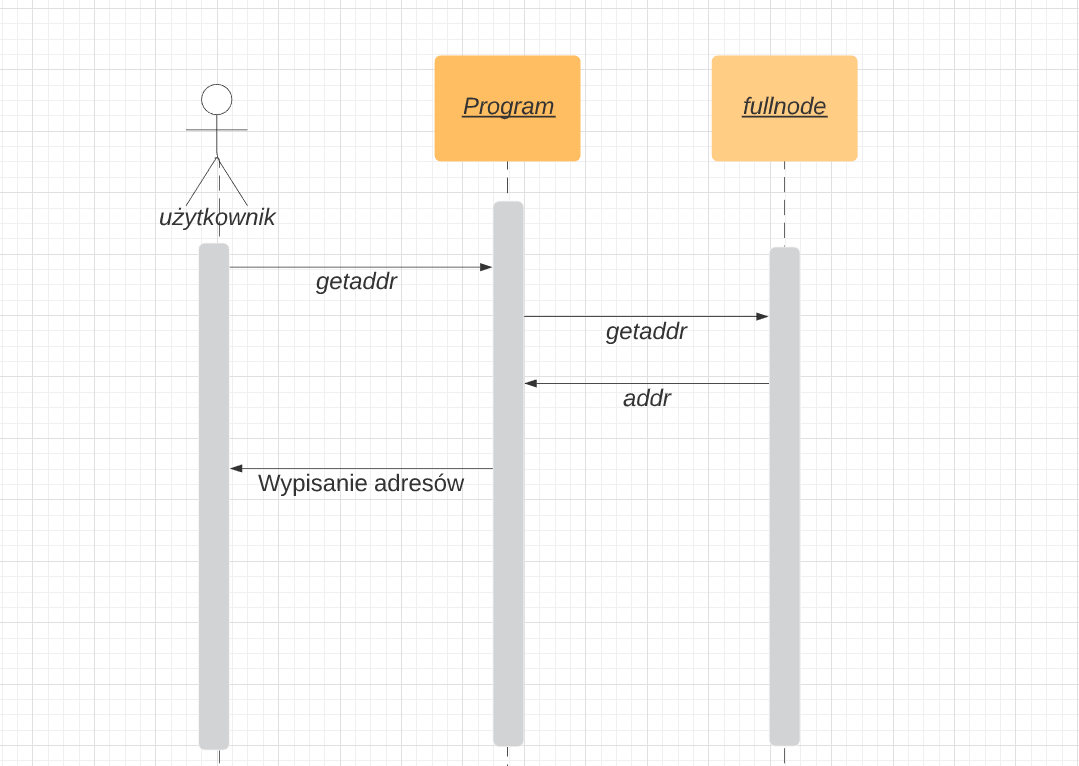
\includegraphics[width=\textwidth]{zdjecia/sekwencjiGetAddr}
\end{figure}

\begin{figure}

\caption{Diagram sekwencji dla nawiązywania połączenia(version,verack).}
\label{zdj:sek:version}
\centering
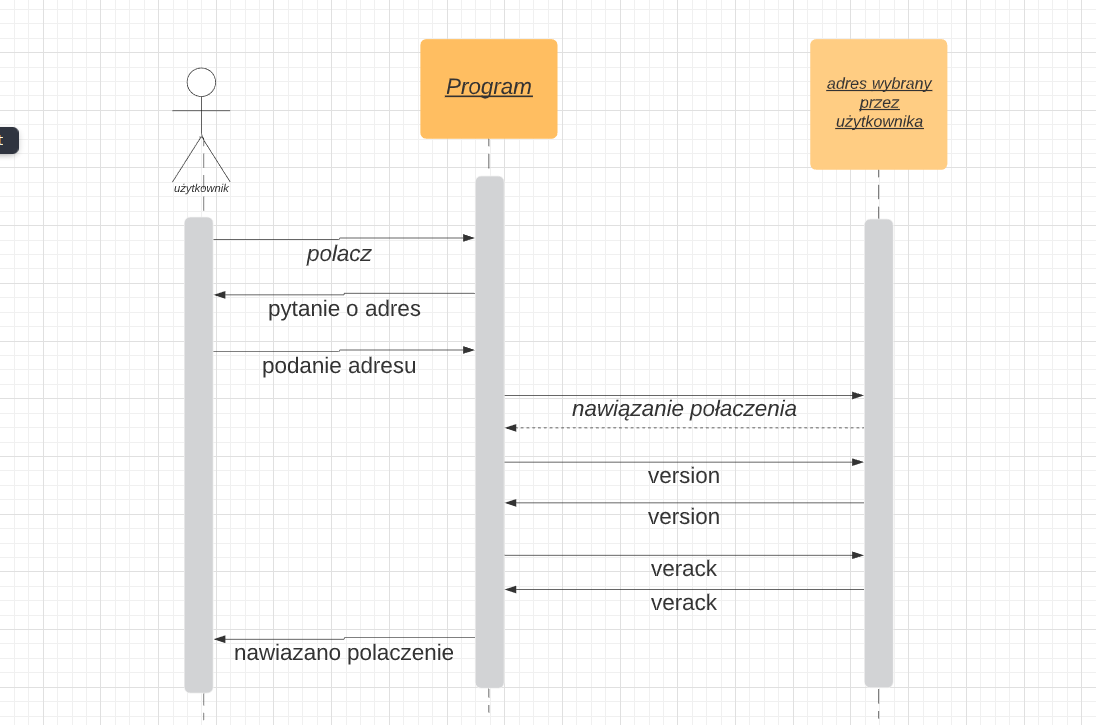
\includegraphics[width=\textwidth]{zdjecia/sekwencjiVersion}
\end{figure}
\end{document}